%%%%%%%%%%%%%%%%%%%% file editor.tex %%%%%%%%%%%%%%%%%%%%%%%%%%%%%%%
%
% sample root file for a complete "contributed book"
%
% "contributed book"
%
% Copy it to a new file with a new name and
% use it as a template for your own input.
%
%%%%%%%%%%%%%%%%%%%%%%%% Springer-Verlag %%%%%%%%%%%%%%%%%%%%%%%%%%


\documentclass{svmult}

% choose options for [] as required from the list
% in the Reference Guide, Sect. 2.2

\usepackage{makeidx}         % allows index generation
\usepackage{graphicx}        % standard LaTeX graphics tool
                             % when including figure files
\usepackage{multicol}        % used for the two-column index
\usepackage[bottom]{footmisc}% places footnotes at page bottom
% etc.
% see the list of further useful packages
% in the Reference Guide, Sects. 2.3, 3.1-3.3

\makeindex             % used for the subject index
                       % please use the style sprmidx.sty with
                       % your makeindex program


%%%%%%%%%%%%%%%%%%%%%%%%%%%%%%%%%%%%%%%%%%%%%%%%%%%%%%%%%%%%%%%%%%%%%

\begin{document}



\frontmatter%%%%%%%%%%%%%%%%%%%%%%%%%%%%%%%%%%%%%%%%%%%%%%%%%%%%%%


%%%%%%%%%%%%%%%%%%%%%%% dedic.tex %%%%%%%%%%%%%%%%%%%%%%%%%%%%%%%%%
%
% sample dedication
%
% Use this file as a template for your own input.
%
%%%%%%%%%%%%%%%%%%%%%%%% Springer-Verlag %%%%%%%%%%%%%%%%%%%%%%%%%%

\thispagestyle{empty}
\vspace*{3.5cm}
\begin{flushright}

% write your text here
{\large Your dedication goes here}

\end{flushright}




%%%%%%%%%%%%%%%%%%%%%%%%%%%%%%%%%%%%%%%%%%%%%%%%%%%%%%%%%%%%%%%
% sample preface
%
% Copy it to a new file with a new name and use it as the basis
% for your article
%
%%%%%%%%%%%%%%%%%%%%%%%% Springer-Verlag %%%%%%%%%%%%%%%%%%%%%%%%%%

\preface

%% Please write your preface here
Here come the golden words

\vspace{1cm}
\begin{flushright}\noindent
place(s),\hfill {\it Firstname  Surname}\\
month year\hfill {\it Firstname  Surname}\\
\end{flushright}




\tableofcontents

%%%%%%%%%%%%%%%%%%%% file editor.tex %%%%%%%%%%%%%%%%%%%%%%%%%%%%%%%
%
% sample file for a complete "list of contributors"
%
% Copy it to a new file with a new name and
% use it as a template for your own input.
%
% please note that this environment makes use of the
% "obeylines"-function.
%
%%%%%%%%%%%%%%%%%%%%%%%% Springer-Verlag %%%%%%%%%%%%%%%%%%%%%%%%%%
\begin{thecontriblist}
\textbf{Author Name}
University/Institute Name
Street No.
X - Place, Postal Code
\texttt{name@e-mail.*}
\and
\textbf{Author Name}
University/Institute Name
Street No.
X - Place, Postal Code
\texttt{name@e-mail.*}
\and
\textbf{Author Name}
University/Institute Name
Street No.
X - Place, Postal Code
\texttt{name@e-mail.*}
\and
\textbf{Author Name}
University/Institute Name
Street No.
X - Place, Postal Code
\texttt{name@e-mail.*}
\and
\textbf{Author Name}
University/Institute Name
Street No.
X - Place, Postal Code
\texttt{name@e-mail.*}
\and
\textbf{Author Name}
University/Institute Name
Street No.
X - Place, Postal Code
\texttt{name@e-mail.*}
\and
\textbf{Author Name}
University/Institute Name
Street No.
X - Place, Postal Code
\texttt{name@e-mail.*}
\and
\textbf{Author Name}
University/Institute Name
Street No.
X - Place, Postal Code
\texttt{name@e-mail.*}
\and
\textbf{Author Name}
University/Institute Name
Street No.
X - Place, Postal Code
\texttt{name@e-mail.*}
\and
\textbf{Author Name}
University/Institute Name
Street No.
X - Place, Postal Code
\texttt{name@e-mail.*}
\and
\textbf{Author Name}
University/Institute Name
Street No.
X - Place, Postal Code
\texttt{name@e-mail.*}
\and
\textbf{Author Name}
University/Institute Name
Street No.
X - Place, Postal Code
\texttt{name@e-mail.*}
\and
\textbf{Author Name}
University/Institute Name
Street No.
X - Place, Postal Code
\texttt{name@e-mail.*}
\and
\textbf{Author Name}
University/Institute Name
Street No.
X - Place, Postal Code
\texttt{name@e-mail.*}
\and
\textbf{Author Name}
University/Institute Name
Street No.
X - Place, Postal Code
\texttt{name@e-mail.*}
\and
\textbf{Author Name}
University/Institute Name
Street No.
X - Place, Postal Code
\texttt{name@e-mail.*}
\and
\textbf{Author Name}
University/Institute Name
Street No.
X - Place, Postal Code
\texttt{name@e-mail.*}
\and
\textbf{Author Name}
University/Institute Name
Street No.
X - Place, Postal Code
\texttt{name@e-mail.*} \and
\textbf{Author Name}
University/Institute Name
Street No.
X - Place, Postal Code
\texttt{name@e-mail.*}
\and
\textbf{Author Name}
University/Institute Name
Street No.
X - Place, Postal Code
\texttt{name@e-mail.*} \and
\textbf{Author Name}
University/Institute Name
Street No.
X - Place, Postal Code
\texttt{name@e-mail.*}
\and
\textbf{Author Name}
University/Institute Name
Street No.
X - Place, Postal Code
\texttt{name@e-mail.*}
\end{thecontriblist}


\mainmatter%%%%%%%%%%%%%%%%%%%%%%%%%%%%%%%%%%%%%%%%%%%%%%%%%%%%%%%
%%%%%%%%%%%%%%%%%%%%%%%%%%%%%%%%%%%%%%%%%%%%%%%%%%%%%%%%%%%%%%%
% sample part title
%
% Copy it to a new file with a new name and use it
% use it as a template for your own input.
%
%%%%%%%%%%%%%%%%%%%%%%%% Springer-Verlag %%%%%%%%%%%%%%%%%%%%%%%%%%


\part{Part Title}

%%%%%%%%%%%%%%%%%%%%%%%%%% author.tex %%%%%%%%%%%%%%%%%%%%%%%%%
%
% sample root file for your contribution to a
%
% "contributed book" (global)
%
% Use this file as a template for your own input.
%
%%%%%%%%%%%%%%%%%%%%%%%% Springer-Verlag %%%%%%%%%%%%%%%%%%%%%%%%%%


%%% The following preamble of the contribution has been commented out
%%% to allow LaTeX to \include that document into the main book

% RECOMMENDED %%%%%%%%%%%%%%%%%%%%%%%%%%%%%%%%%%%%%%%%%%%%%%%%%%%
%\documentclass{svmult}

%% choose options for [] as required from the list
%% in the Reference Guide, Sect. 2.2

%\usepackage{makeidx}         % allows index generation
%\usepackage{graphicx}        % standard LaTeX graphics tool
                              % when including figure files
%\usepackage{multicol}        % used for the two-column index
%\usepackage[bottom]{footmisc}% places footnotes at page bottom
% etc.
% see the list of further useful packages
% in the Reference Guide, Sects. 2.3, 3.1-3.3

%\makeindex             % used for the subject index
                       % please use the style sprmidx.sty with
                       % your makeindex program


%%%%%%%%%%%%%%%%%%%%%%%%%%%%%%%%%%%%%%%%%%%%%%%%%%%%%%%%%%%%%%%%%%%%%

%\begin{document}

\title*{Contribution Title}
% Use \titlerunning{Short Title} for an abbreviated version of
% your contribution title if the original one is too long
\author{Name of Author\inst{1}\and
Name of Author\inst{2}}
% Use \authorrunning{Short Title} for an abbreviated version of
% your contribution title if the original one is too long
\institute{Name and Address of your Institute
\texttt{name@email.address}
\and Name and Address of your Institute \texttt{name@email.address}}
%
% Use the package "url.sty" to avoid
% problems with special characters
% used in your e-mail or web address
%
\maketitle

Your text goes here. Separate text sections with the standard \LaTeX\
sectioning commands.

\section{Section Heading}
\label{sec:1}
% Always give a unique label
% and use \ref{<label>} for cross-references
% and \cite{<label>} for bibliographic references
% use \sectionmark{}
% to alter or adjust the section heading in the running head
Your text goes here. Use the \LaTeX\ automatism for your citations
\cite{monograph}.

\subsection{Subsection Heading}
\label{sec:2}
Your text goes here.

\begin{equation}
\vec{a}\times\vec{b}=\vec{c}
\end{equation}

\subsubsection{Subsubsection Heading}
Your text goes here. Use the \LaTeX\ automatism for cross-references as
well as for your citations, see Sect.~\ref{sec:1}.

\paragraph{Paragraph Heading} %
Your text goes here.

\subparagraph{Subparagraph Heading.} Your text goes here.%
%
\index{paragraph}
% Use the \index{} command to code your index words
%
% For tables use
%
\begin{table}
\center
\caption{Please write your table caption here}
\label{tab:1}       % Give a unique label
%
% For LaTeX tables use
%
\begin{tabular}{lll}
\hline\noalign{\smallskip}
first & second & third  \\
\noalign{\smallskip}\hline\noalign{\smallskip}
number & number & number \\
number & number & number \\
\noalign{\smallskip}\hline
\end{tabular}
\end{table}
%
%
% For figures use
%
\begin{figure}
\center
% Use the relevant command for your figure-insertion program
% to insert the figure file.
% For example, with the option graphics use
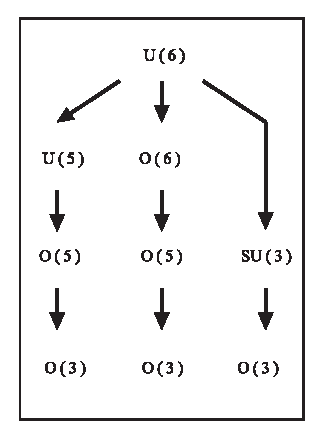
\includegraphics[height=4cm]{figure.eps}
%
% If not, use
%\picplace{5cm}{2cm} % Give the correct figure height and width in cm
%
\caption{Please write your figure caption here}
\label{fig:1}       % Give a unique label
\end{figure}
%
% For built-in environments use
%
\begin{theorem}
Theorem text\footnote{Footnote} goes here.
\end{theorem}
%
% or
%
\begin{lemma}
Lemma text goes here.
\end{lemma}
%
%
% BibTeX users please use
% \bibliographystyle{}
% \bibliography{}
%
% Non-BibTeX users please follow the syntax
% the syntax of "referenc.tex" for your own citations
%%%%%%%%%%%%%%%%%%%%%%%% referenc.tex %%%%%%%%%%%%%%%%%%%%%%%%%%%%%%
% sample references
% "engineering"
%
% Use this file as a template for your own input.
%
%%%%%%%%%%%%%%%%%%%%%%%% Springer-Verlag %%%%%%%%%%%%%%%%%%%%%%%%%%

%
% BibTeX users please use
% \bibliographystyle{}
% \bibliography{}
%
% Non-BibTeX users please use
\begin{thebibliography}{99.}
%
% and use \bibitem to create references.
%
% Use the following syntax and markup for your references
%
% Monographs
\bibitem{monograph} Kipphan H (2000)
Handbook of printmedia. Springer, Berlin Heidelberg New York

% Contributed Works
\bibitem{contribution} Brandt J, Hein W (2001) Polymer materials in
joint surgery. In: Grellmann~W, Seidler S (eds)
Deformation and fracture behavior of polymers. Engineering
materials. Springer, Berlin Heidelberg New York

% Journal
\bibitem{journal} Che M, Grellmann W, Seidler S (1997)
Appl Polym Sci 64:1079--1090

% Theses
\bibitem{thesis} Ross DW (1977) Lysosomes and storage diseases. MA
Thesis, Columbia University, New York

\end{thebibliography}

%%%%%%%%%%%%%%%%%%%%%%%%%%%%%%%%%%%%%%%%%%%%%%%%%%%%%%%%%%%%%%%%%%%%%%

%\printindex
%\end{document}






%%%%%%%%%%%%%%%%%%%%%%%%%% author.tex %%%%%%%%%%%%%%%%%%%%%%%%%
%
% sample root file for your contribution to a
%
% "contributed book" (global)
%
% Use this file as a template for your own input.
%
%%%%%%%%%%%%%%%%%%%%%%%% Springer-Verlag %%%%%%%%%%%%%%%%%%%%%%%%%%


%%% The following preamble of the contribution has been commented out
%%% to allow LaTeX to \include that document into the main book

% RECOMMENDED %%%%%%%%%%%%%%%%%%%%%%%%%%%%%%%%%%%%%%%%%%%%%%%%%%%
%\documentclass{svmult}

%% choose options for [] as required from the list
%% in the Reference Guide, Sect. 2.2

%\usepackage{makeidx}         % allows index generation
%\usepackage{graphicx}        % standard LaTeX graphics tool
                              % when including figure files
%\usepackage{multicol}        % used for the two-column index
%\usepackage[bottom]{footmisc}% places footnotes at page bottom
%% etc.
%% see the list of further useful packages
%% in the Reference Guide, Sects. 2.3, 3.1-3.3

%\makeindex             % used for the subject index
                       % please use the style sprmidx.sty with
                       % your makeindex program


%%%%%%%%%%%%%%%%%%%%%%%%%%%%%%%%%%%%%%%%%%%%%%%%%%%%%%%%%%%%%%%%%%%%%

%\begin{document}

\title*{Contribution Title}
% Use \titlerunning{Short Title} for an abbreviated version of
% your contribution title if the original one is too long
\author{Name of Author\inst{1}\and
Name of Author\inst{2}}
% Use \authorrunning{Short Title} for an abbreviated version of
% your contribution title if the original one is too long
\institute{Name and Address of your Institute
\texttt{name@email.address}
\and Name and Address of your Institute \texttt{name@email.address}}
%
% Use the package "url.sty" to avoid
% problems with special characters
% used in your e-mail or web address
%
\maketitle

Your text goes here. Separate text sections with the standard \LaTeX\
sectioning commands.

\section{Section Heading}
\label{sec:1b}
% Always give a unique label
% and use \ref{<label>} for cross-references
% and \cite{<label>} for bibliographic references
% use \sectionmark{}
% to alter or adjust the section heading in the running head
Your text goes here. Use the \LaTeX\ automatism for your citations
\cite{monograph}.

\subsection{Subsection Heading}
\label{sec:2b}
Your text goes here.

\begin{equation}
\vec{a}\times\vec{b}=\vec{c}
\end{equation}

\subsubsection{Subsubsection Heading}
Your text goes here. Use the \LaTeX\ automatism for cross-references as
well as for your citations, see Sect.~\ref{sec:1b}.

\paragraph{Paragraph Heading} %
Your text goes here.

\subparagraph{Subparagraph Heading.} Your text goes here.%
%
\index{paragraph}
% Use the \index{} command to code your index words
%
% For tables use
%
\begin{table}
\center
\caption{Please write your table caption here}
\label{tab:1b}       % Give a unique label
%
% For LaTeX tables use
%
\begin{tabular}{lll}
\hline\noalign{\smallskip}
first & second & third  \\
\noalign{\smallskip}\hline\noalign{\smallskip}
number & number & number \\
number & number & number \\
\noalign{\smallskip}\hline
\end{tabular}
\end{table}
%
%
% For figures use
%
\begin{figure}
\center
% Use the relevant command for your figure-insertion program
% to insert the figure file.
% For example, with the option graphics use
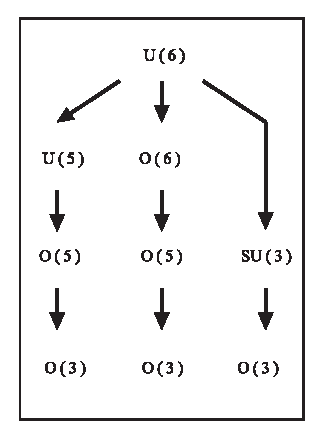
\includegraphics[height=4cm]{figure.eps}
%
% If not, use
%\picplace{5cm}{2cm} % Give the correct figure height and width in cm
%
\caption{Please write your figure caption here}
\label{fig:1b}       % Give a unique label
\end{figure}
%
% For built-in environments use
%
\begin{theorem}
Theorem text\footnote{Footnote} goes here.
\end{theorem}
%
% or
%
\begin{lemma}
Lemma text goes here.
\end{lemma}
%
%
% BibTeX users please use
% \bibliographystyle{}
% \bibliography{}
%
% Non-BibTeX users please follow the syntax
% the syntax of "referenc.tex" for your own citations
%%%%%%%%%%%%%%%%%%%%%%%% referenc.tex %%%%%%%%%%%%%%%%%%%%%%%%%%%%%%
% sample references
% "engineering"
%
% Use this file as a template for your own input.
%
%%%%%%%%%%%%%%%%%%%%%%%% Springer-Verlag %%%%%%%%%%%%%%%%%%%%%%%%%%

%
% BibTeX users please use
% \bibliographystyle{}
% \bibliography{}
%
% Non-BibTeX users please use
\begin{thebibliography}{99.}
%
% and use \bibitem to create references.
%
% Use the following syntax and markup for your references
%
% Monographs
\bibitem{monograph} Kipphan H (2000)
Handbook of printmedia. Springer, Berlin Heidelberg New York

% Contributed Works
\bibitem{contribution} Brandt J, Hein W (2001) Polymer materials in
joint surgery. In: Grellmann~W, Seidler S (eds)
Deformation and fracture behavior of polymers. Engineering
materials. Springer, Berlin Heidelberg New York

% Journal
\bibitem{journal} Che M, Grellmann W, Seidler S (1997)
Appl Polym Sci 64:1079--1090

% Theses
\bibitem{thesis} Ross DW (1977) Lysosomes and storage diseases. MA
Thesis, Columbia University, New York

\end{thebibliography}


%%%%%%%%%%%%%%%%%%%%%%%%%%%%%%%%%%%%%%%%%%%%%%%%%%%%%%%%%%%%%%%%%%%%%%

%\printindex
%\end{document}








\backmatter%%%%%%%%%%%%%%%%%%%%%%%%%%%%%%%%%%%%%%%%%%%%%%%%%%%%%%%#
\appendix
%%%%%%%%%%%%%%%%%%%%%%%%%%%%%%%%%%%%%%%%%%%%%%%%%%%%%%%%%%%%%%%
% sample chapter
%
% Copy it to a new file with a new name and use it
% use it as a template for your own input.
%
%%%%%%%%%%%%%%%%%%%%%%%% Springer-Verlag %%%%%%%%%%%%%%%%%%%%%%%%%%

\chapter{Appendix Heading}
\label{A:app} % Give a unique label

Your text comes here. Separate text sections

\section{Section Heading}
\label{A:sec:1}  % Give a unique label
%and use \ref{sec:1} and \cite{journal1}

\subsection{Subsection Heading}
\label{A:sec:2}

\subsubsection{Subsubsection Heading}

\paragraph{Paragraph Heading}
\subparagraph{Subparagraph Heading.} as required%
\index{paragraph}. % Use the \index command for coding your index

% For tables use
%
\begin{table}
\centering
\caption{Please write your table caption here}
\label{A:tab:1}       % Give a unique label
% For LaTeX tables use
\begin{tabular}{lll}
\hline\noalign{\smallskip}
first & second & third  \\
\noalign{\smallskip}\hline\noalign{\smallskip}
number & number & number \\
number & number & number \\
\noalign{\smallskip}\hline
\end{tabular}
\end{table}
%
%
% For figures use
%
\begin{figure}
\centering
% Use the relevant command for your figure-insertion program
% to insert the figure file.
% For example, with the option graphics use
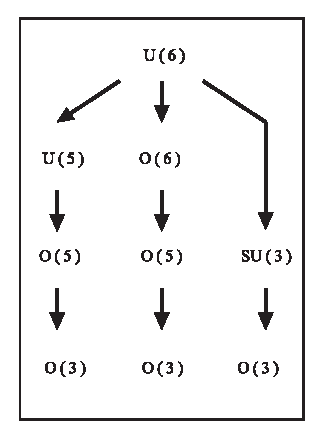
\includegraphics[height=3cm]{figure.eps}
% If not, use
%\picplace{5cm}{2cm} % Give the correct figure height and width in cm
\caption{Please write your figure caption here}
\label{A:fig:1}       % Give a unique label
\end{figure}



\printindex

%%%%%%%%%%%%%%%%%%%%%%%%%%%%%%%%%%%%%%%%%%%%%%%%%%%%%%%%%%%%%%%%%%%%%%

\end{document}





